\chapter{Metodologías}
\label{chap:metodologias}

\drop{H}{  ubo} un tiempo en el que desarrollar un juego no necesitaba mucho más de un equipo pequeño de personas (3 ó 4 como máximo) y no mucho más de 6 meses de esfuerzo \cite{dill-07}, pero la exacerbada competencia que existe actualmente en la industria implica equipos de desarrollo de más de 50 personas expertas trabajando durante varios años con un presupuesto de millones de dólares para lograr publicar un solo videojuego comercial \cite{mor-10}. 

Por tanto, dada la evidente complejidad tanto técnica como personal de un videojuego, es necesario manejar su desarrollo haciendo uso de las metodologías y técnicas de planificación adecuadas que involucren una serie de pasos organizados para guiar cada proceso hasta el resultado final; es decir, hacer un buen uso de la \textbf{Ingeniería del Software}. Según describe el ingeniero americano Barry Bohem en \cite{Boe-79}, un artículo de referencia en este campo, la Ingeniería del Software es \textit{the practical application of scientific knowledge to the design and the construction of computer programs and the associated documentation required to develop, operate and maintain them}.

Tras leer esta definición es fácil darse cuenta de lo fundamental que es llevar a cabo un diseño e implementación adecuados. En este capítulo se hablará de la metodología de desarrollo de videojuegos más común y a continuación se presenta y justificará la metodología de trabajo seguida a lo largo del desarrollo de \textit{MineRVa}.

\section{Metodologías de desarrollo de videojuegos}

Los videojuegos no dejan de ser un recurso informático, aunque están muy próximos en cuanto a consumo y producción al entorno audiovisual. El sistema de producción audiovisual tiene clara relación con gran parte de las fases de desarrollo del videojuego pero, a pesar de ser considerado un software más, no existe una metodología común y propia para su diseño y desarrollo \cite{man-14}. El campo del videojuego ya no es sólo una industria que aporta importantes beneficios sino que se convierte en objeto de estudio en lo que a metodologías se refiere \cite{agu-08}.

El desarrollo de un juego, a lo largo de su ciclo de vida, se puede asemejar al de una película de cine, pudiéndose segmentar en tres fases ampliamente diferenciadas: \textbf{pre-producción}, \textbf{producción} y \textbf{post-producción}, cada una con sus etapas características \cite{bet-03}.

\vspace{0.4cm}

\begin{figure}[!h]
    \begin{center}
        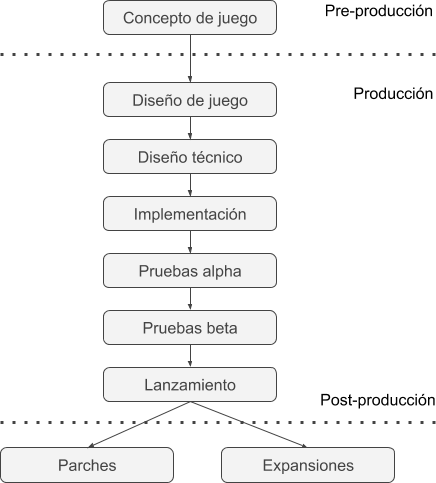
\includegraphics[width=0.625\textwidth]{imagenes/5/pre-prod-post.png}
        \caption{Fases del desarrollo de videojuegos, adaptado de \cite{man-14}}
        \label{fig:fases-desarrollo}
    \end{center}
\end{figure}

Esta metodología puede ser usada con distintos procesos de desarrollo, como \textit{Rational Unified Process}, \textit{Scrum} o \textit{Huddle}. Este último es un proceso específico de desarrollo de videojuegos y se llama así siguiendo la analogía de Scrum, ya que la reunión que se realiza en el fútbol americano antes de cada jugada se llama \textit{huddle}. Su filosofía es que mediante breves reuniones se planifique cada iteración, permitiendo tanto realizar un seguimiento más específico al avance del proyecto como poder hacer correcciones tempranas ante posibles desviaciones \cite{mor-10}.

Aunque el problema de proyectos privativos como videojuegos a gran escala es que no suele filtrarse mucha información referente a su parte técnica, sí se sabe que uno de los procesos más populares ha sido el de Cascada, aunque poco a poco las compañías han ido migrando a metodologías de desarrollo ágiles, más flexibles \cite{mor-10}.

A continuación se explican estas fases con más profundidad.

\subsection{Fase de pre-producción}

En la primera fase del proyecto se define el concepto de juego que estamos buscando así como sus aspectos más relevantes, como su \textbf{género}, su \textbf{historia} y sus principales \textbf{bocetos} para obtener una primera idea de su estilo \cite{rou-05}. Además, en esta fase se comienza a dar forma al \acs{GDD}, del que ya se habló en el capítulo \ref{chap:analisis_problema}.

\subsection{Fase de producción}

Esta es la fase más exigente del proyecto. En ella participan multitud de profesionales muy especializados y confluyen toda clase de actividades, como el diseño técnico, el diseño artístico o el diseño mecánico y la implementación y pruebas de los mismos. 

Además, a lo largo de esta fase se generan muchos documentos . Los más importantes son el \acs{GDD}, cuya finalización debería coincidir con la de esta fase, y la \textbf{Biblia del juego}, donde se recogen todas las historias de los personajes, del mundo donde sucede el juego, de su pasado y de los personajes secundarios que aparecen, creando el hilo argumental completo, con todos los detalles \cite{man-14}.

Esta fase termina con la generación del \textbf{gold master}, la copia definitiva que se envía a fábrica para su producción junto con el arte como la portada o el manual de usuario.

\subsection{Fase de post-producción}

Pero como ya sabemos el ciclo de vida de un producto software no termina con su entrega o, en este caso, su lanzamiento al mercado. Además de las tareas de marketing pertinentes, será preciso llevar a cabo un seguimiento adecuado para dar respuesta al comportamiento que el mercado ha tenido en relación al juego, ya que puede llegar a ser muy diferente al esperado.

Las tareas más inmediatas pueden ser parches para arreglar elementos o para ajustar su funcionamiento, y si nuestro juego contempla el lanzamiento de expansiones o DLCs (\textit{downloadable content}) también deberemos hacerlo en esta fase. Además, también deberá realizarse un \textbf{análisis post-portem} del proyecto para saber qué ha ido mal y poder mejorarlo para futuros proyectos.

Como puede verse, el desarrollo de un videojuego es una tarea larga y extremadamente compleja en la que intervienen profesionales de todo tipo y que es orquestada por un equipo de dirección que se encarga de que todo vaya según lo planeado y otro equipo de financiación encargado de que el presupuesto de producción se cumpla \cite{man-14}.

\section{Metodología de trabajo}

Antes de presentar el proceso de desarrollo y la metodología de desarrollo utilizada en este proyecto se describirá lo que es cada uno.

Un \textbf{proceso de desarrollo} es una representación abstracta de una metodología de desarrollo. Procesos de desarrollo como por ejemplo \acs{UDP} o \textit{Agile Development} son abstracciones que definen las actividades que deben realizarse, pero no especifican cómo realizarlas o cuál debería ser el resultado.

Por otro lado, una \textbf{metodología de desarrollo} es la implementación específica de un proceso de desarrollo. Ejemplos de eso son \acs{RUP}, \textit{eXtreme Programming} y \textit{Scrum}. No son completamente explícitos pero definen qué, cuándo y cómo hacer las cosas.

Una vez diferenciados ambos conceptos, se pasa a explicar el proceso y la metodología de desarrollo que ha seguido este \acs{TFM}.

\subsection{Proceso de desarrollo}

En vista de los requisitos de flexibilidad que propone, y que en un proyecto de esta naturaleza son especialmente importantes, se ha elegido seguir el \textbf{Agile Software Development}.

Los principios fundamentales que rigen el Desarrollo Ágil están expuestos en \textbf{The Manifesto for Agile Software Development}\footnote{\url{http://agilemanifesto.org/}}, que fue escrito en febrero de 2001 por diecisiete ingenieros de software que llegaron a un acuerdo acerca de los cuatro pilares básicos que definían la forma correcta de desarrollar software.

\begin{center}
\begin{tcolorbox}[sharp corners,  colframe=white]
\begin{enumerate}
    \item \textbf{Individuals and interactions} over processes and tools.
    \item \textbf{Working software} over comprehensive documentation.
    \item \textbf{Customer collaboration} over contract negotiation.
    \item \textbf{Responding to change} over following a plan.
\end{enumerate}
\end{tcolorbox}
\end{center}

La primera regla hace referencia a la importancia del factor humano y a su coordinación, y asigna un papel secundario a seguir la metodología del proyecto de manera invariable.

La segunda regla señala la necesidad de priorizar el software resultante y su funcionalidad y utilidad sobre una documentación exhaustiva del proyecto.

La tercera regla da a entender a la importancia de colaborar con el cliente tanto como sea posible, en lugar de firmar un documento estático al comienzo del proyecto que contenga todos sus requisitos y no aceptar nada que no apareciera inicialmente en él.

Por último, la cuarta regla se enfoca en tratar de tomar decisiones flexibles ante problemas repentinos y cambios no planificados, adaptando el proyecto a ellos, en lugar de tratar de seguir el plan inicial a toda costa.

Del mismo modo, se definieron \textbf{12 principios}\footnote{\url{http://agilemanifesto.org/principles.html}} explicando qué debe regir cada metodología de desarrollo de software que utiliza este proceso de desarrollo.

\subsection{Metodología de desarrollo}

Dadas las necesidades de desarrollo explicadas anteriormente, la metodología de desarrollo más cercana a ellas es \textbf{Scrum}. Scrum no es una técnica para la construcción de productos; en su lugar, es un marco en el que se pueden emplear varios procesos y técnicas. Por este motivo Scrum no es una metodología exclusiva de desarrollo de software, ya que puede aplicarse a otras áreas, se adapta muy bien y permite que el equipo sea flexible para abordar los problemas y lograr resultados de alto valor \cite{scrum-guide}.

El principal valor de Scrum es su alta adaptabilidad a los cambios, lo que permite que el equipo y la organización del proyecto respondan rápidamente a los nuevos requisitos. Estos enfoques serían imposibles aplicando otras metodologías, como por ejemplo la de desarrollo en cascada.

Scrum se basa en la teoría empírica de control de procesos, que afirma que el conocimiento proviene de la experiencia y la toma de decisiones basadas en lo que se conoce. Esta metodología se apoya en tres pilares básicos.

\begin{itemize}
    \item \textbf{Transparencia.} Cualquier acción significativo debe ser visible para cada persona en el proyecto. Solo de este modo se puede compartir una comprensión común de lo que está sucediendo en cualquier momento.
    
    \item \textbf{Inspección.} Los artefactos de Scrum deben ser inspeccionados para detectar resultados indeseados. Estas inspecciones serán más beneficiosas si son realizadas por inspectores cualificados y siempre que no sean tan frecuentes como para interferir en el trabajo.

    \item \textbf{Adaptación}. Scrum utiliza un enfoque iterativo e incremental para adaptarse a los cambios y para controlar los riesgos. Cuando se detecte un problema, estas adaptaciones se deben realizar lo antes posible para desviarse lo menos posible de la planificación inicial.
\end{itemize}

Etimológicamente, \textit{scrum} es un movimiento en Rugby en el que un equipo se reúne para actuar de manera coordinada para que el balón pase de un extremo del campo al otro opuesto. Por lo tanto, hasta el nombre de esta metodología apunta a la necesidad de trabajar como un equipo sincronizado y bien comunicado para lograr un objetivo común.

De esta manera, Scrum intenta evitar que haya momentos en que un miembro del equipo no sepa qué hacer o no aporte valor al desarrollo, aunque Dilbert, en la figura \ref{fig:dilbert}, no esté de acuerdo con esto.

\begin{figure}[!h]
\begin{center}
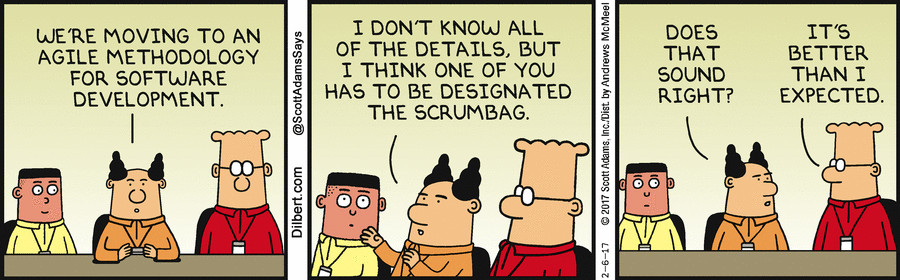
\includegraphics[width=0.95\textwidth]{imagenes/5/dilbert.jpg}
\caption{Dilbert y los roles de equipo, de \url{https://dilbert.com}}
\label{fig:dilbert}
\end{center}
\end{figure}

\subsubsection{Artefactos y eventos}

La figura \ref{fig:scrum} presenta una visión general de cómo funciona el flujo de trabajo de Scrum.

\begin{figure}[!h]
\begin{center}
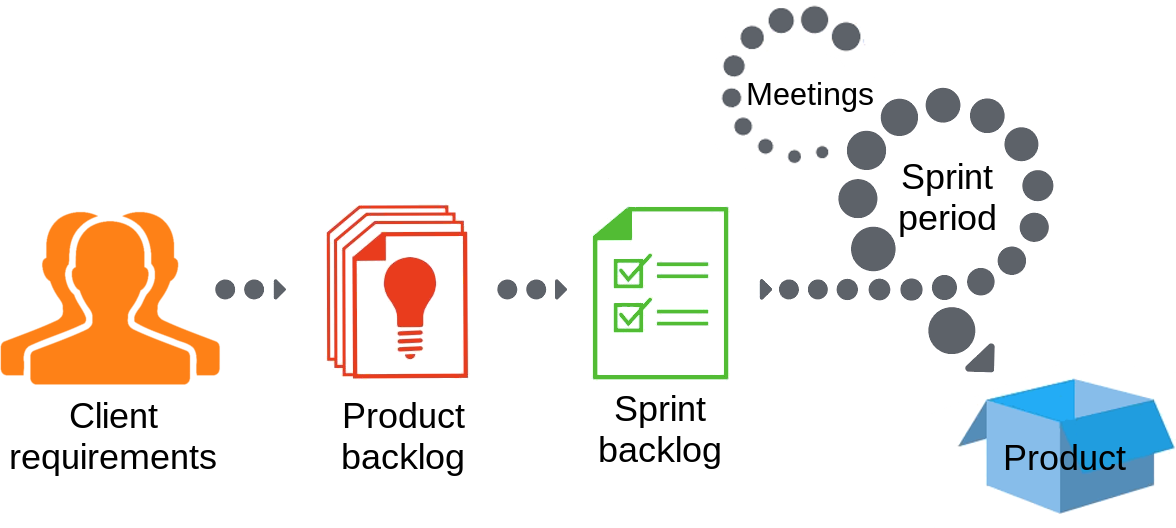
\includegraphics[width=0.95\textwidth]{imagenes/5/scrum.png}
\caption{Flujo de trabajo de Scrum, adaptado de \url{https://www.scrumalliance.org}}
\label{fig:scrum}
\end{center}
\end{figure}

Para poder explicar los roles de Scrum más claramente, primero se describirán brevemente los eventos que forman parte de esta metodología \cite{scrum-guide}.

\begin{itemize}
\item \textbf{Product backlog.} La cartera del producto es una abstracción que sirve para controlar las \textbf{historias de usuario} o \textit{user stories}. Éstas reflejan los requisitos que debe satisfacer el proyecto, que son establecidos por el cliente o el propietario del producto. 

Pero el \textit{product backlog} no solo permite agregar historias de usuarios, sino también todas las características, funciones y soluciones a las necesidades del proyecto. Cada uno de ellas estará formado por una descripción, una prioridad y el valor que agrega al producto. Además, se puede añadir el miembro Scrum asignado para completarla y cualquier observación relevante.

El \textit{product backlog} nunca se cierra, por lo que desde el inicio hasta el cierre del proyecto se pueden añadir nuevas historias de usuario o se pueden eliminar las que ya existen. Por lo tanto, a medida que el proyecto avanza la lista tiende crecen y alcanzan su máximo justo antes de la entrega final. Los requisitos nunca dejan de evolucionar, por lo que el \textit{product backlog} es un \textbf{objeto vivo}. Los cambios en los requisitos comerciales, las condiciones del mercado o la tecnología pueden hacer que cambie.
    
\item \textbf{Sprint.} El concepto clave de Scrum es un sprint, una \textbf{fase de trabajo} que dura un máximo de un mes, lo que genera un nuevo artefacto que puede ser potencialmente integrado en el producto final.

Se debe evitar que el tiempo del sprint sea demasiado largo, ya que de lo contrario la definición de lo que se está construyendo se vuelve demasiado amplia y la complejidad  y el riesgo aumentan.

Cada sprint puede considerarse un proyecto autocontenido, ya que se utilizan para lograr objetivos. Cada sprint tiene una definición de lo que se construirá, un diseño y un plan flexible que guiará su construcción y el artefacto resultante. Un nuevo sprint comienza inmediatamente después de que el anterior termine.

Un sprint está formado por varios eventos y artefactos.

\begin{itemize}

    \item [$\circ$] \textbf{Sprint period.} Es el período de tiempo que el sprint está destinado a durar.
        
    \item [$\circ$] \textbf{Sprint planning meeting.} Es una reunión dirigida por el \textbf{scrum master}, que debe asegurarse de que cada miembro haya entendido correctamente el resultado de la reunión.
    
    Esta reunión, que se lleva a cabo al comienzo de cada sprint, permite planear el trabajo a realizar de forma colaborativa por parte del equipo Scrum a partir del \textit{product backlog}.
    
    \item [$\circ$] \textbf{Sprint backlog.} Es un conjunto de elementos que pertenecen al \textit{product backlog} y que han sido \textbf{seleccionados para el sprint actual}. Es un pronóstico realizado por el equipo sobre qué funcionalidad estará en el próximo \textbf{incremento}. El \textit{sprint backlog} puede contener más de un solo elemento; de hecho, el equipo de Scrum añade los elementos identificados como necesarios para cumplir con el objetivo del sprint.
    
    Existen varias técnicas destinadas a lidiar con la necesidad de predecir cuánto puede durar una historia de usuario, como los \textbf{Mapa de afinidad} o el \textbf{Planning Poker}. Esta última es una técnica de estimación basada en el consenso dedicada a ayudar al equipo de desarrollo a tomar una decisión coordinada. Cada miembro hará una predicción en base a algunos valores prefijados y la representará el tiempo que cree que puede llevar terminar cada historia de usuario. Si todo el mundo coincide se dará por buena, pero si no se discutirá y se repetirá la votación hasta que todo el mundo coincida\footnote{\url{https://www.mountaingoatsoftware.com/agile/planning-poker}}.
        
    \item [$\circ$] \textbf{Daily Scrum.} Es un evento de 15 minutos para que el \textbf{equipo de desarrollo sincronice sus actividades} y cree un plan para el día actual. Esto se hace mirando el trabajo desde el último Scrum diario y prediciendo el trabajo que podría realizarse antes del siguiente. A lo largo de esta reunión, cada miembro del equipo responderá a tres preguntas:
    
    \begin{enumerate}
    \item ¿Qué hice ayer?
    \item ¿Qué voy a hacer hoy?
    \item ¿Creo que hay algo que está dificultando el desarrollo?
    \end{enumerate}
    
    De esa modo es muy fácil saber exactamente qué está haciendo cada miembro del equipo y detectar problemas emergentes.
    
     \item [$\circ$] \textbf{Sprint review.} Es una reunión informal que se lleva a cabo al final de cada sprint para \textbf{inspeccionar el trabajo realizado} y actualizar el \textit{product backlog}. La duración de ésta reunión suele ser directamente proporcional a la duración del sprint.
     
     \item [$\circ$] \textbf{Sprint retrospective.} Esta reunión se lleva a cabo después del \textit{sprint review} y antes de la planificación del próximo sprint, y ayuda al equipo de Scrum a inspeccionar el trabajo realizado y \textbf{detecte puntos débiles} antes del el próximo sprint.
        
\end{itemize}

\item \textbf{Product.} Es el motivo por el cual se desarrolla el proyecto; el artefacto final que se entregará al cliente.

\end{itemize}

\subsubsection{Flujo de trabajo y roles}

El marco trabajo de Scrum consta de varios roles; el \textbf{product owner} o propietario del producto, el \textbf{Scrum master} o maestro Scrum, \textbf{equipo de desarrollo} y los \textbf{stakeholders} o interesados, quienes juntos forman el \textbf{Scrum team}. Cada rol se relaciona con los otros por medio de varias actividades, eventos, interacciones y artefactos, y cada uno tiene un propósito específico y es esencial para el éxito del proyecto. Estas funciones y sus interacciones se muestran a continuación \cite{scrum-card}.

\begin{itemize}
\item \textbf{Product owner.} Es el responsable de \textbf{maximizar el valor del producto} coordinando correctamente las relaciones del Scrum team. Además, es el único responsable de administrar el \textit{product backlog}, lo que incluye,

\begin{itemize}
    \item[$\circ$] Definir las \textbf{historias de usuario}.
    \item[$\circ$] Ordenar las \textbf{historias de usuario} para alcanzar los objetivos de la mejor manera posible.
    \item[$\circ$] Asegurarse de que el \textit{product backlog} sea visible, transparente y \textbf{claro para todo el mundo}.
\end{itemize}

\item \textbf{Scrum master.} Es el responsable de garantizar que la \textbf{metodología Scrum sea entendida y aplicada por todo el mundo}. El Scrum master debe actuar como líder al servicio del equipo Scrum y ayudar a aumentar el valor de los artefactos que genere. 

El Scrum master puede ayudar a cada rol a maximizar su valor de varias maneras:
 
\begin{itemize}
    \item[$\circ$] \textbf{Al \textit{product owner}.} Su interacción principal con el este rol está dirigida a garantizar la gestión adecuada del \textit{product backlog}, haciendo que las historias de usuario sean lo más claras posible.
    
    \item[$\circ$] \textbf{Al equipo de desarrollo.} El Scrum master debe liderar al equipo de desarrollo y aumentar su efectividad para que generen productos de alto valor.
    
    \item[$\circ$] \textbf{A la organización.} El Scrum master debe ayudar a todas las partes interesadas a comprender y aplicar Scrum y trabajar con otros Scrum masters de otros equipos para aumentar la efectividad de la aplicación de esta metodología dentro de la organización.
    
\end{itemize}

\item \textbf{Equipo de desarrollo.} Que está formado por los desarrolladores que entregan el trabajo al cliente. Solo los miembros del equipo de desarrollo pueden crear el incrementos en el producto y decir que una historia de usuario se ha completado.

Estos desarrolladores son \textbf{auto-organizados} y \textbf{multi-función}. Además, Scrum no reconoce sub-equipos dentro del equipo de desarrollo. Aunque los miembros individuales pueden tener habilidades especializadas y áreas de enfoque, la responsabilidad del producto pertenece al equipo de desarrollo en su conjunto.

\item \textbf{Stakeholders.} Los interesados pueden ser individuos o empresas que se ven afectados por activa o por pasiva por el desarrollo del proyecto.

\end{itemize}

\section{Conclusiones y aplicación de las metodologías}

Como se ha visto, las metodologías de desarrollo de videojuegos son complejas, ya que requieren la sincronización y el trabajo conjunto de muchos profesionales. Sin embargo, en este proyecto solo ha trabajado una persona, por lo que se han simplificado estas metodologías, adaptándolas a los requisitos del proyecto. Una de las principales ventajas de utilizar metodologías ágiles es esto mismo; poder modelar los procesos de desarrollo a las necesidades del proyecto a medida. 

Como en los entornos reales de desarrollo de videojuegos, este proyecto se ha desarrollo en torno a su \acs{GDD}, el documento que contiene toda su información, lo que significa que las iteraciones y el trabajo que conllevan se han basado en él.

Para ello, se ha diseñado un plan de entregas que guíe estas iteraciones y del que se hablará en el capítulo \ref{chap:plan_entregas}. Como se indica en Scrum, el final de cada iteración debe estar marcado por la generación de un entregable. Para probarlo, al final de cada iteración se grabará un vídeo mostrando los avances obtenidos a lo largo de la misma, que durará entre 4 y 6 minutos, y se subirá a YouTube. Además, en el capítulo \ref{chap:desarrollo}, que habla del desarrollo del proyecto a través de sus iteraciones, se mostrarán estos vídeos y se indicará su URL para que el lector pueda verlos y comprobar que su fecha de subida concuerda con la de su iteración.

Además, tanto el proyecto como su documentación se alojarán en repositorios de GitHub, cuyos respectivos enlaces son los siguientes.

\begin{center}
    \url{https://github.com/gomezportillo/mineRVa}
    \url{https://github.com/gomezportillo/mineRVa-doc}
\end{center}
